% Copyright 2004 by Till Tantau <tantau@users.sourceforge.net>.
%
% In principle, this file can be redistributed and/or modified under
% the terms of the GNU Public License, version 2.
%
% However, this file is supposed to be a template to be modified
% for your own needs. For this reason, if you use this file as a
% template and not specifically distribute it as part of a another
% package/program, I grant the extra permission to freely copy and
% modify this file as you see fit and even to delete this copyright
% notice. 

\documentclass{beamer}
\usepackage{etex}

\usepackage[utf8]{inputenc}
\usepackage[spanish]{babel}
\usepackage{lmodern}

\usepackage{graphicx}

\usepackage{multicol}
\usepackage{mathtools}
\usepackage{hyperref}
\usepackage{listings}
\usepackage{verbatim}
\usepackage{afterpage}
\usepackage{lscape}

\usepackage{multirow, array} % para las tablas

\usepackage{amsmath}

\usepackage{cite}


% Gráficos, tablas, etc.
\usepackage{pgfplots, pgfplotstable, booktabs, colortbl, siunitx, array}

\usepackage{media9}


%\usepackage{multimedia}
\sisetup{table-auto-round}

% Establecemos el tema a utilizar. 
% Debe existir el archivo udpthesisEIT.sty en su sistema TeX para poder utilizarlo.

%%%%%%%%%%%%%%%%%%%%%%%%%%%%%%%
\usepackage{xspace}
\makeatletter
\DeclareRobustCommand\onedot{\futurelet\@let@token\@onedot}
\def\@onedot{\ifx\@let@token.\else.\null\fi\xspace}

\def\eg{\emph{e.g}\onedot} \def\Eg{\emph{E.g}\onedot}
\def\ie{\emph{i.e}\onedot} \def\Ie{\emph{I.e}\onedot}
\def\cf{\emph{c.f}\onedot} \def\Cf{\emph{C.f}\onedot}
\def\etc{\emph{etc}\onedot} \def\vs{\emph{vs}\onedot}
\def\wrt{w.r.t\onedot} \def\dof{d.o.f\onedot}
\def\etal{\emph{et al}\onedot}
\def\adhoc{\emph{ad hoc}\xspace}
\makeatother

\usepackage{amsthm}
% declare my operator
\usepackage{scalerel}
\DeclareMathOperator*{\cat}{\scalerel*{\|}{\sum}}



% There are many different themes available for Beamer. A comprehensive
% list with examples is given here:
% http://deic.uab.es/~iblanes/beamer_gallery/index_by_theme.html
% You can uncomment the themes below if you would like to use a different
% one:
%\usetheme{AnnArbor}
%\usetheme{Antibes}
%\usetheme{Bergen}
%\usetheme{Berkeley}
%\usetheme{Berlin}
%\usetheme{Boadilla}
%\usetheme{boxes}
%\usetheme{CambridgeUS}
%\usetheme{Copenhagen}
%\usetheme{Darmstadt}
%\usetheme{default}
%\usetheme{Frankfurt}
%\usetheme{Goettingen}
%\usetheme{Hannover}
%\usetheme{Ilmenau}
%\usetheme{JuanLesPins}
%\usetheme{Luebeck}
\usetheme{Madrid}
%\usetheme{Malmoe}
%\usetheme{Marburg}
%\usetheme{Montpellier}
%\usetheme{PaloAlto}
%\usetheme{Pittsburgh}
%\usetheme{Rochester}
%\usetheme{Singapore}
%\usetheme{Szeged}
%\usetheme{Warsaw}

\setbeamertemplate{footline}[page number]{}
\setbeamertemplate{bibliography item}{[\theenumiv]}

\title{Reconocimiento de expresiones faciales en imágenes dinámicas utilizando un descriptor basado en rayos de flujo}

% A subtitle is optional and this may be deleted
%\subtitle{Optional Subtitle}

\author{Miguel Antonio Rodríguez Santander}
% - Give the names in the same order as the appear in the paper.
% - Use the \inst{?} command only if the authors have different
%   affiliation.

\institute[Universidad Diego Portales] % (optional, but mostly needed)
{%
  Universidad Diego Portales\\
  Facultad de Ingeniería\\
  Escuela de Informática y Telecomunicaciones
  
  % - Use the \inst command only if there are several affiliations.
% - Keep it simple, no one is interested in your street address.
}
\date{Título II\\ 5 de Diciembre de 2015}
% - Either use conference name or its abbreviation.
% - Not really informative to the audience, more for people (including
%   yourself) who are reading the slides online

\subject{Thesis}
% This is only inserted into the PDF information catalog. Can be left
% out. 

% If you have a file called "university-logo-filename.xxx", where xxx
% is a graphic format that can be processed by latex or pdflatex,
% resp., then you can add a logo as follows:

% \pgfdeclareimage[height=0.5cm]{university-logo}{university-logo-filename}
% \logo{\pgfuseimage{university-logo}}

% Delete this, if you do not want the table of contents to pop up at
% the beginning of each subsection:

\AtBeginSection[]
{
  \begin{frame}<beamer>{Índice}
    \tableofcontents[currentsection,currentsubsection]
  \end{frame}
}

%\AtBeginSubsection[]
%{
%  \begin{frame}<beamer>{Índice}
%    \tableofcontents[currentsection,currentsubsection]
%  \end{frame}
%}

% Let's get started
\begin{document}

\begin{frame}
  \titlepage
\end{frame}

\begin{frame}{Índice}
  \tableofcontents
  % You might wish to add the option [pausesections]
\end{frame}

% Section and subsections will appear in the presentation overview
% and table of contents.


% You can reveal the parts of a slide one at a time
% with the \pause command:

\section{Motivación}

\begin{frame}
  \frametitle{Motivación}
  \begin{columns}[onlytextwidth]
    \begin{column}{0.5\textwidth}
      \centering
      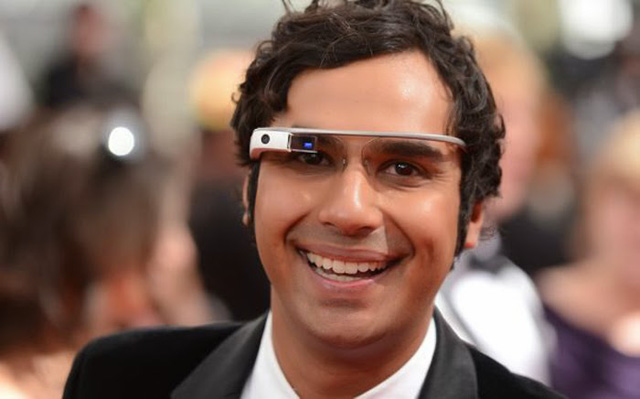
\includegraphics[width=5cm]{imagenes/google_glass.jpg}
    \end{column}
    \begin{column}{0.5\textwidth}
        \begin{itemize}
            \item Aplicaciones a distintas áreas del conocimiento humano
            \item Utilidad en tecnologías actuales
            \item 55\% en la transmisión del mensaje
        \end{itemize}
    \end{column}
  \end{columns}
\end{frame}


\section{Problema}
    
    \begin{frame}{Problema}{Expresiones faciales universales}
		  \begin{columns}[onlytextwidth]
    		  	\begin{column}{0.7\textwidth}
      			\centering
      			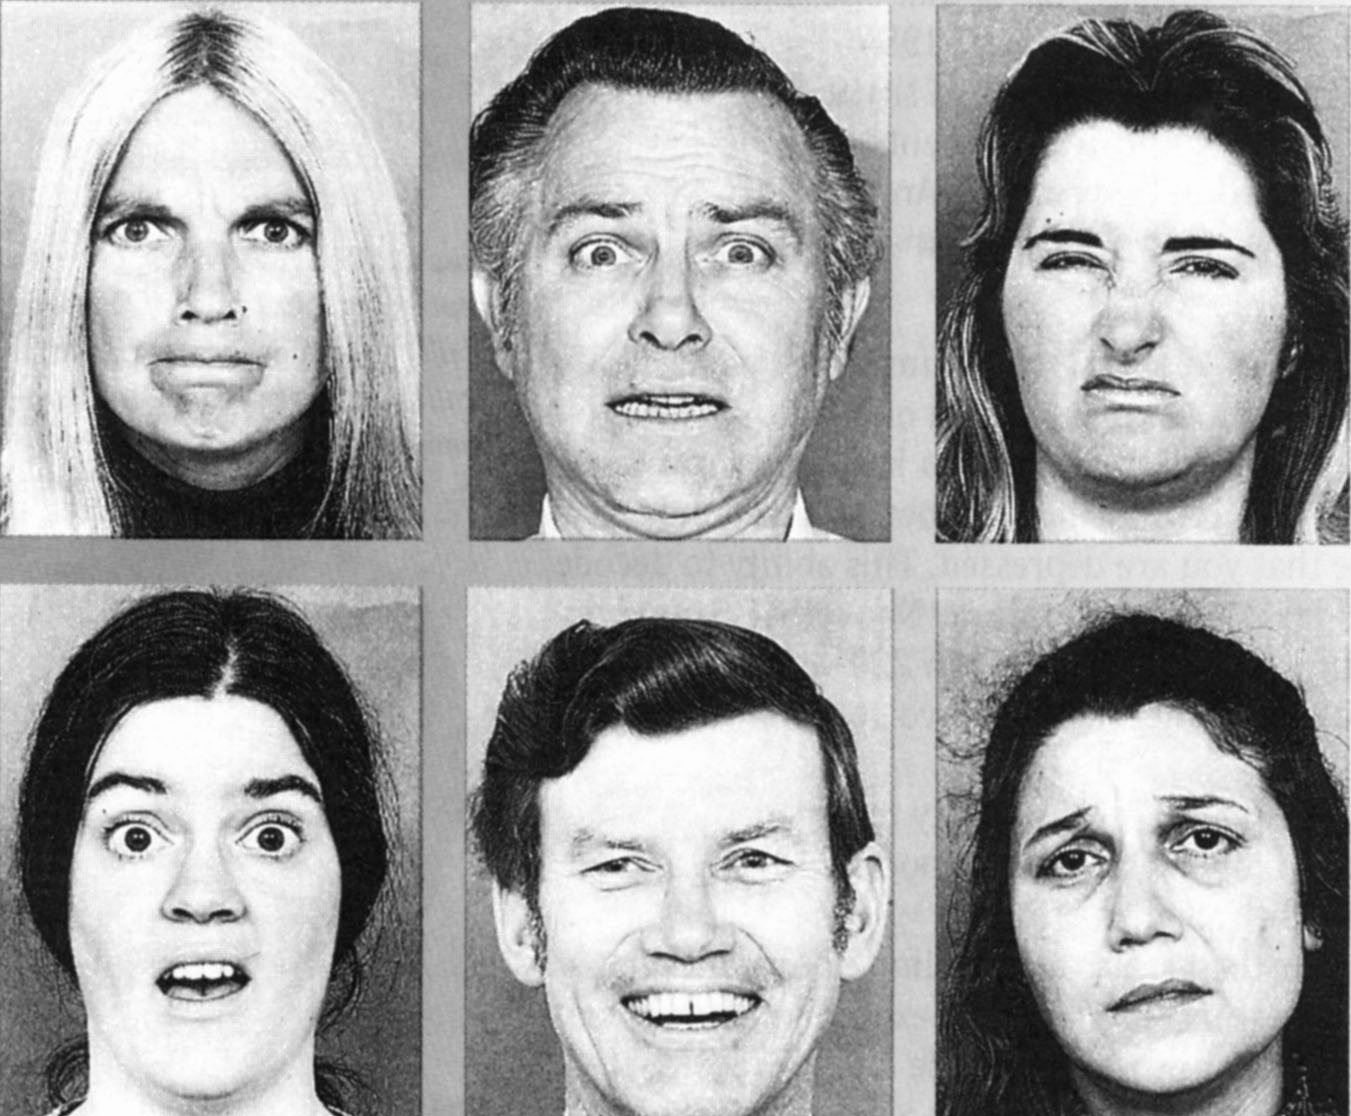
\includegraphics[width=7cm]{imagenes/expresiones_faciales_universales.jpg}
    			\end{column}
    		    \begin{column}{0.3\textwidth}
        	      \begin{itemize}
            	    \item Alegría
            		\item Asco
            		\item Ira
            		\item Miedo
            		\item Sorpresa
            		\item Tristeza
        	   	  \end{itemize}
            \end{column}
          \end{columns}          
    \end{frame}
    
\section{Solución propuesta}
	\subsection{Pipeline}    
    \begin{frame}{Solución propuesta}{Pipeline}
        \begin{figure}[bt]
    		\centering
            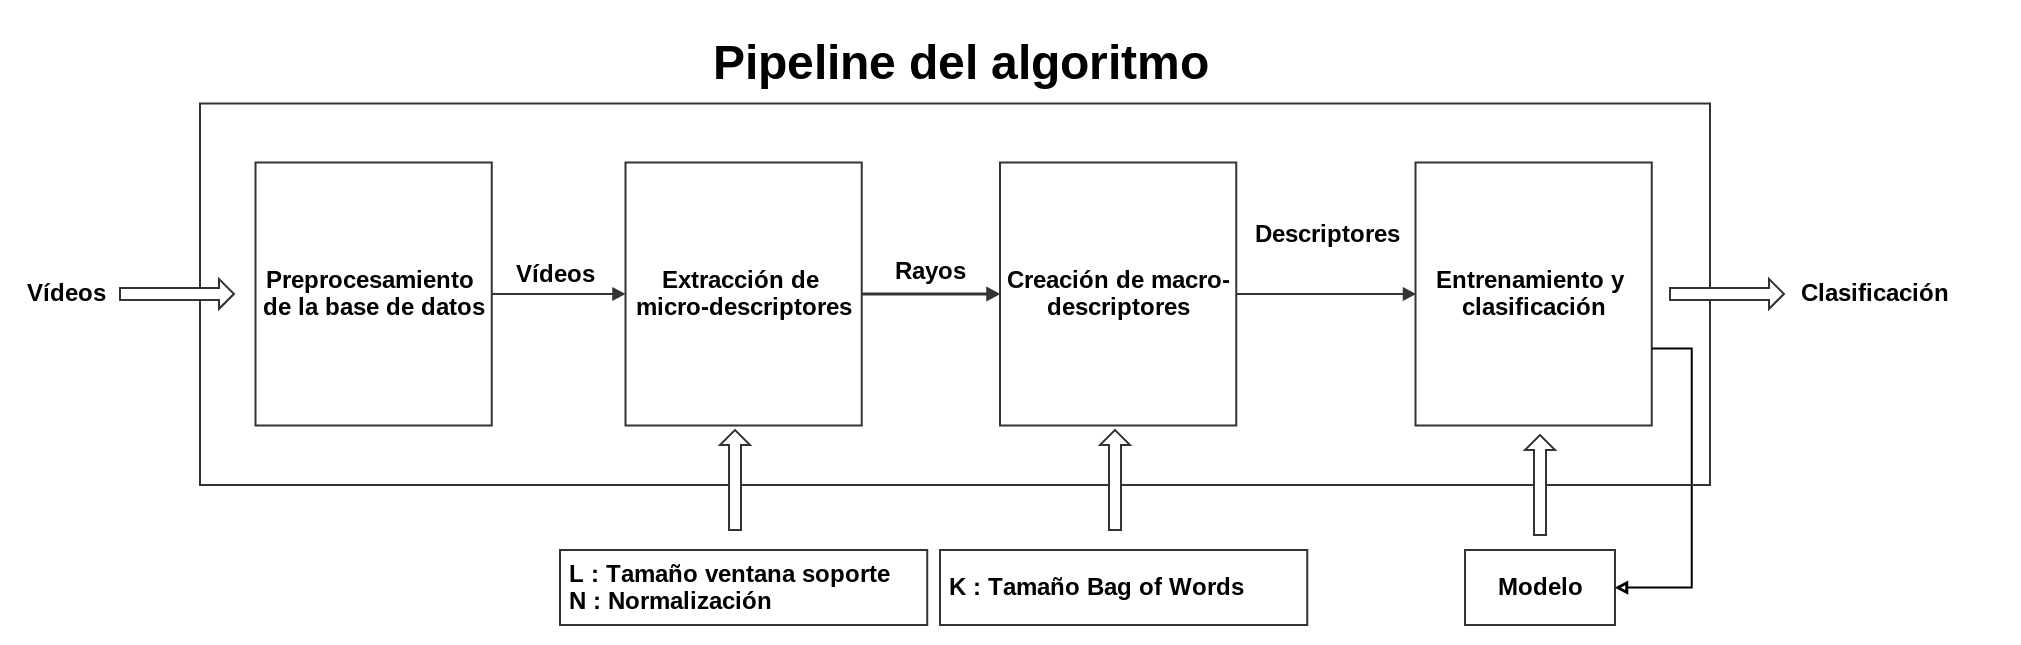
\includegraphics[width=12cm]{imagenes/pipeline.png}
        \end{figure}
    \end{frame}
	
    \subsection{Preprocesamiento de la base de datos}
        \begin{frame}{Preprocesamiento de la base de datos}
        
            \begin{columns}[onlytextwidth]
                \begin{column}{0.4\textwidth}
                    \begin{itemize}
                        \item Detección de rostros
                        \item Corrección de movimiento
                    \end{itemize}
                \end{column}
                \begin{column}{0.6\textwidth}
                    \begin{figure}[bt]
                		\centering
                        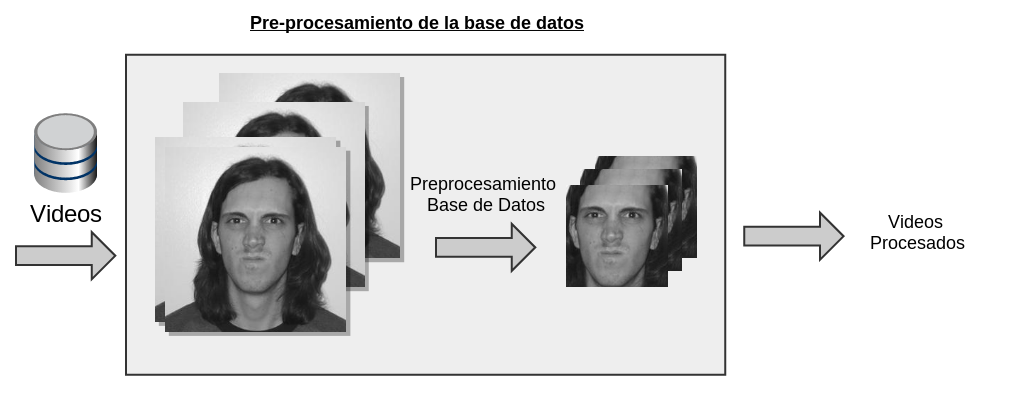
\includegraphics[width=7cm]{imagenes/Preprocesamiento.png}
                    \end{figure}
                \end{column}
            \end{columns}
        
        \end{frame}
    
    
    
    \subsection{Extracción de micro-descriptores}
        \begin{frame}{Extracción de micro-descriptores}{Vista general}
            \begin{figure}[bt]
        		\centering
                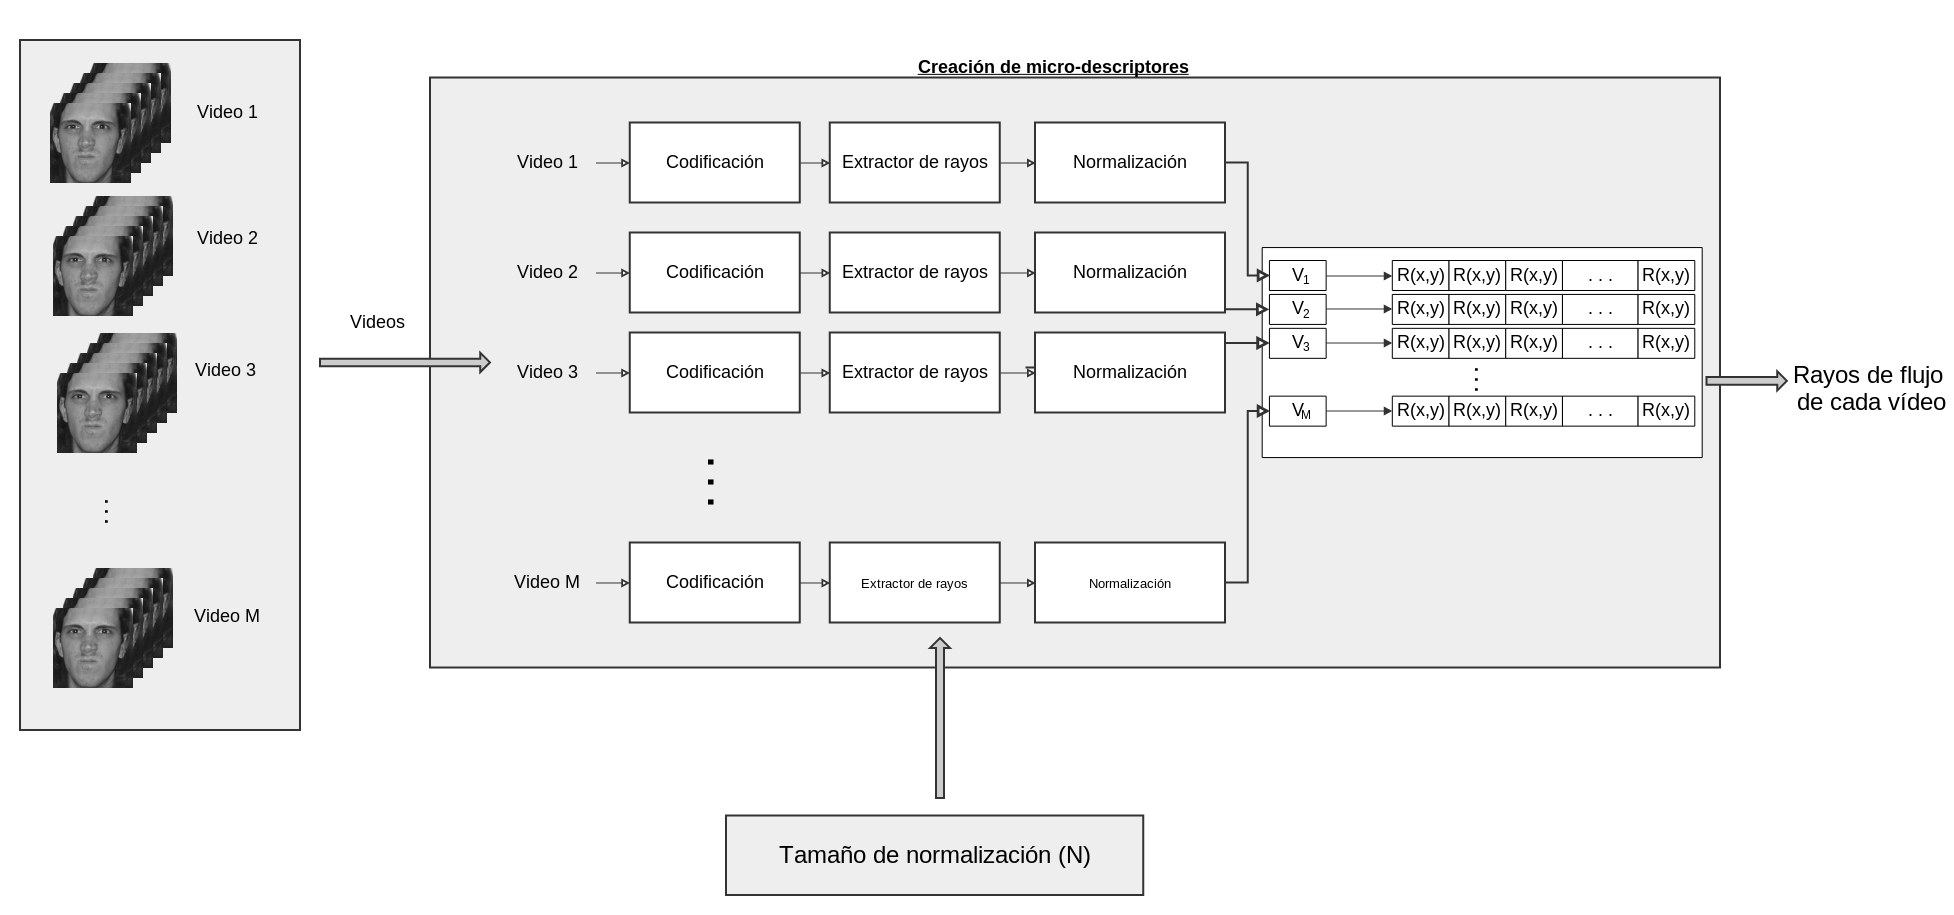
\includegraphics[width=12cm]{imagenes/Extractor_microdescriptores.png}
            \end{figure}
        \end{frame}
    
   		\begin{frame}{Extracción de micro-descriptores}{Codificación: Local Binary Patterns}
   			\begin{figure}[bt]
   				\centering
   				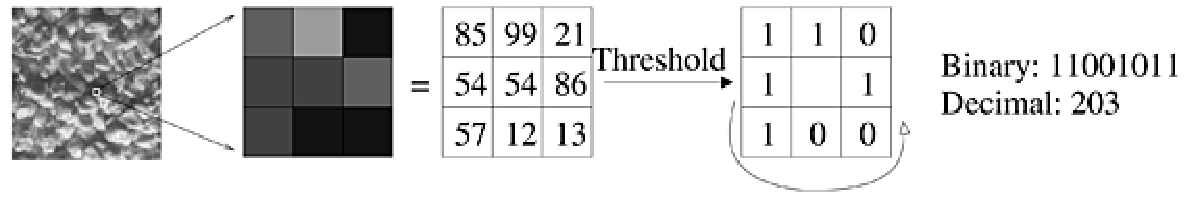
\includegraphics[width=9cm]{imagenes/lbp.pdf}
   			\end{figure}	
   			
   			\begin{figure}[bt]
   				\centering
   				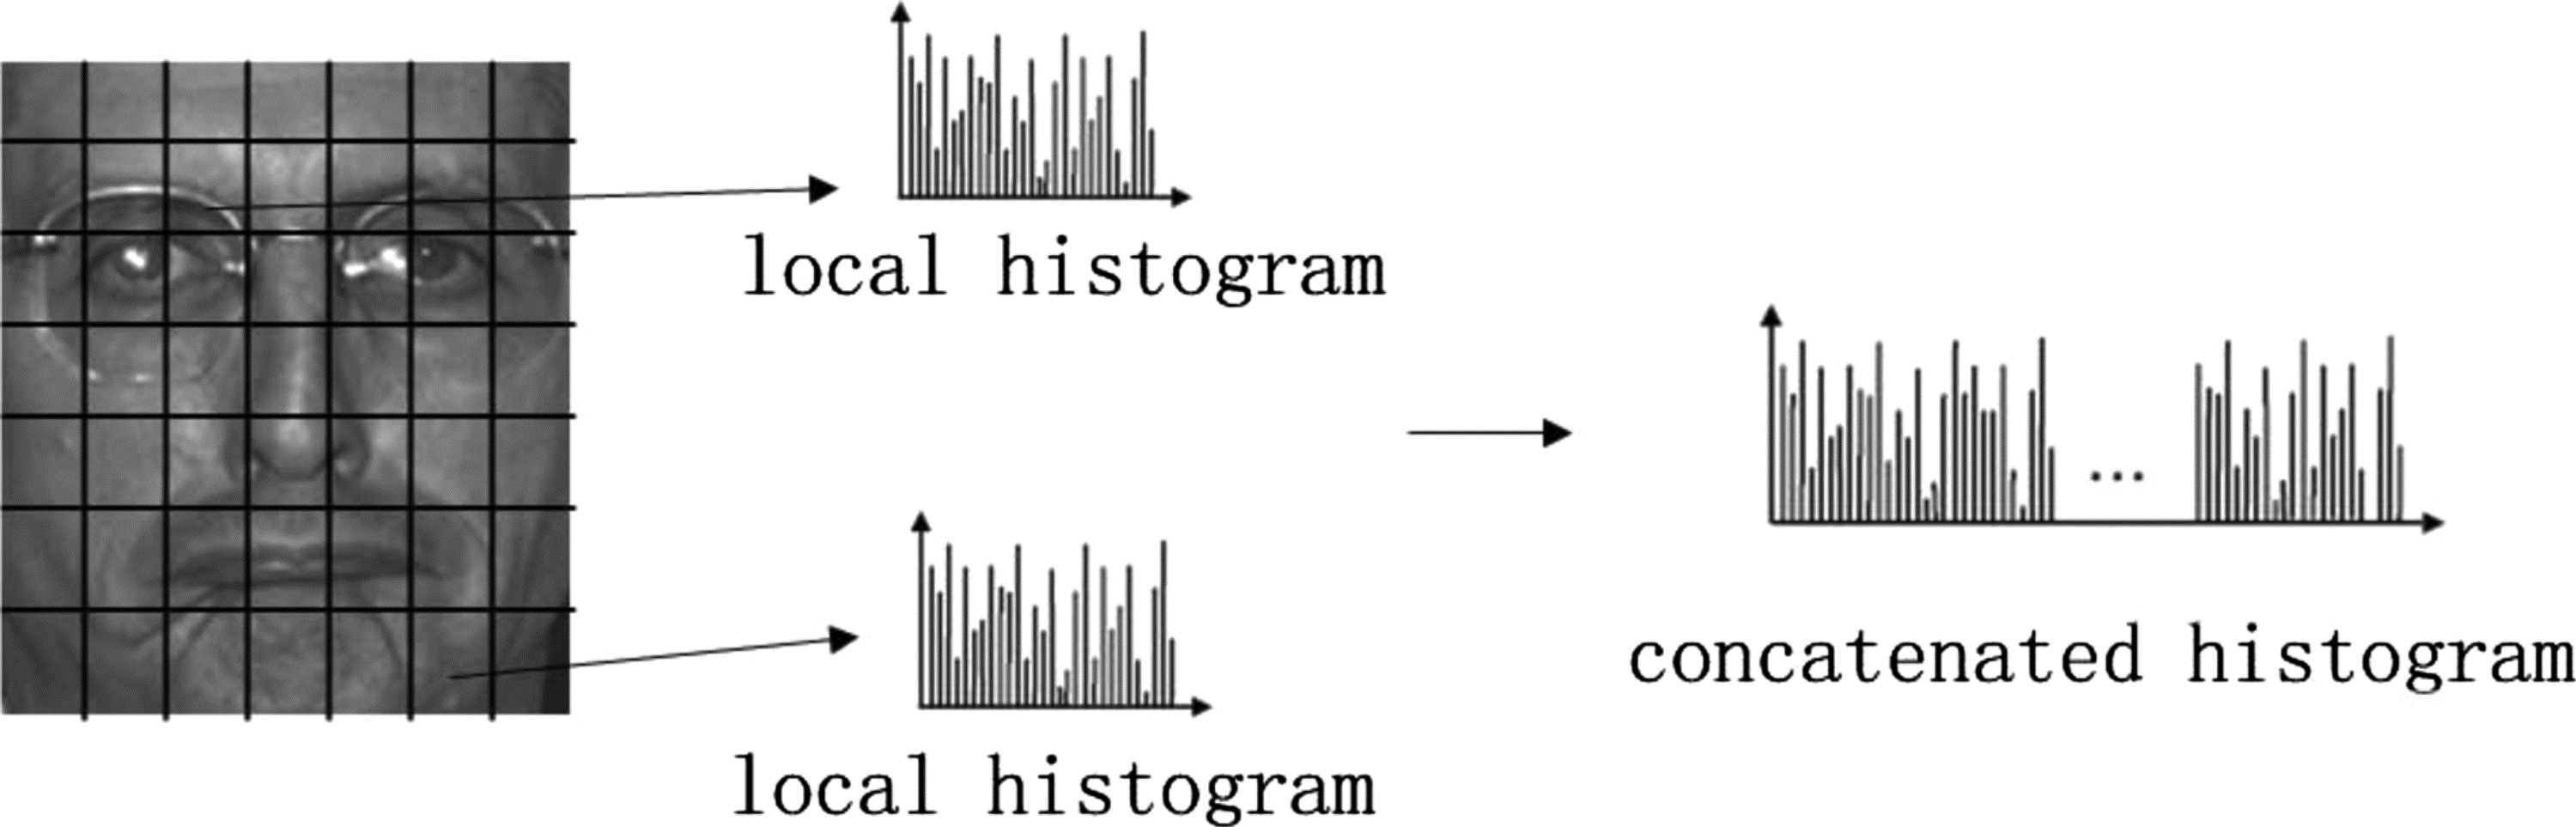
\includegraphics[width=9cm]{imagenes/lbp_histogram.png}
   			\end{figure}	  
   		\end{frame}
    
        \begin{frame}{Extracción de micro-descriptores}{Extracción de rayos}
			\begin{block}{Región de soporte}
            		Región cuadrada de tamaño $R$ centrada en el píxel $(x,y)$ en el tiempo $t$
            \end{block}    			
    			
    			\begin{figure}[bt]
        			\centering
                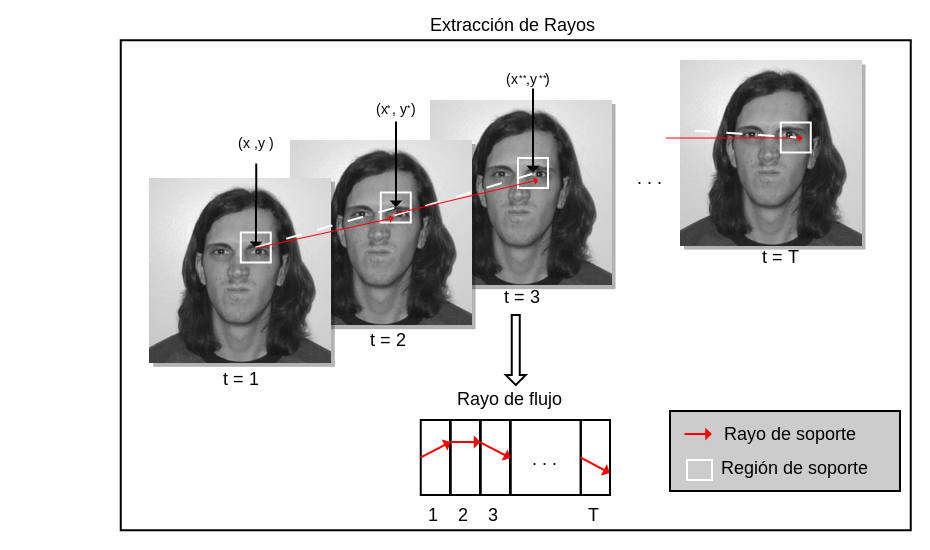
\includegraphics[width=9cm]{imagenes/Extraccion_de_rayos.png}
            \end{figure}        
	        
        \end{frame}
    
    
    		\begin{frame}{Extracción de micro-descriptores}{Extracción de rayos}
			\begin{block}{Ventana de búsqueda}
                  Región cuadrada de tamaño $W$ centrada en el píxel $(x,y)$ en el tiempo $t+1$
            \end{block}    			
    			
    			\begin{figure}[bt]
        			\centering
                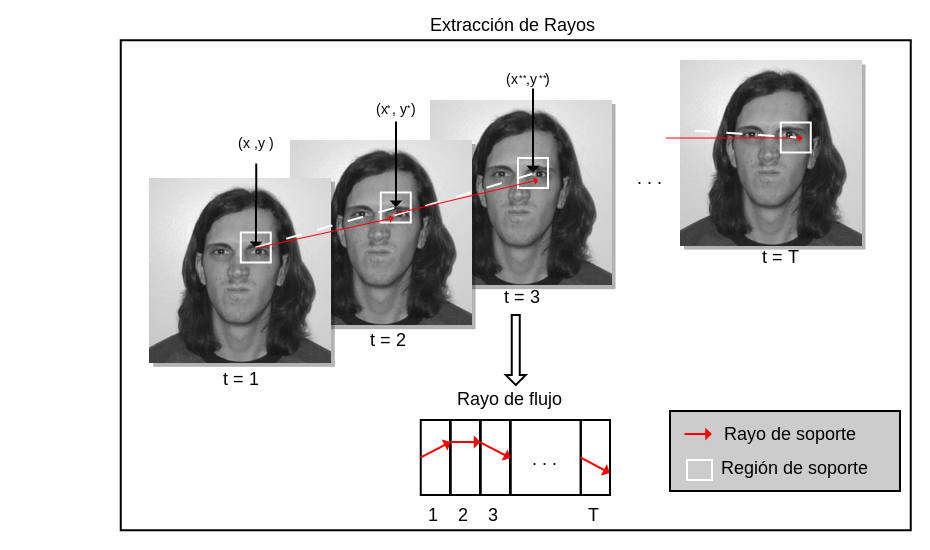
\includegraphics[width=9cm]{imagenes/Extraccion_de_rayos.png}
            \end{figure}        
	            
        \end{frame}
    
        \begin{frame}{Extracción de micro-descriptores}{Extracción de rayos}
			\begin{equation}\label{algoritmo:eq:mse}	
			    \text{MSE}(\text{RS}, \text{RS}') = \sum_{x=1}^{R} \sum_{y=1}^{R} (\text{RS}(x,y,t) - \text{RS}'(x',y', t+1))^2
		    \end{equation}   
		    
		    \begin{equation}
		        \text{RS}^* = \arg \min_{\text{RS}'}\{\text{MSE}(\text{RS},\text{RS}') | \text{RS}' \in \text{WS} \}
	        \end{equation}
	        
	        \begin{columns}[onlytextwidth]
                \begin{column}{0.5\textwidth}
					\begin{figure}[bt]
        					\centering
                			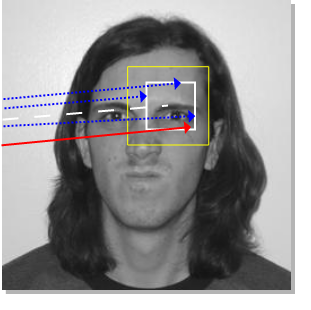
\includegraphics[width=4cm]{imagenes/MSE1.png}
            			\end{figure}      	        	
	        		\end{column}
                \begin{column}{0.5\textwidth}                
                		\begin{table}
                			
					\begin{tabular}{|c|c|}
					                \hline 
					                RS & Región de soporte \\ 
					                \hline 
					                WS & Ventana de búsqueda \\ 
					                \hline 
					                RS' & Subregión de soporte $\in$ WS \\ 
					                \hline 
					                $x$ & Coordenada x del píxel \\ 
					                \hline 
					                $y$ & Coordenada y del píxel \\ 
					                \hline 
					                $\text{RS}^*$ & Subregión óptima $\in$ WS \\
					                \hline 
					 \end{tabular} 
                		\end{table}
	        		\end{column}
	        \end{columns}	
        \end{frame}
        
        
		\begin{frame}{Extracción de micro-descriptores}{Extracción de rayos}
			\begin{block}{Rayo de soporte}
				\begin{equation}
					\rho_{(x,y)} = \{(\Delta x^{t}, \Delta y^{t})~| \forall t\}.
				\end{equation}		 
            \end{block}			
			
			\begin{columns}[onlytextwidth]
                \begin{column}{0.5\textwidth}
					\begin{figure}[bt]
        					\centering
                			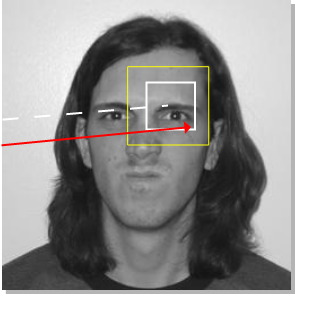
\includegraphics[width=4cm]{imagenes/MSE2.png}
            			\end{figure}      	        	
	        		\end{column}
                \begin{column}{0.5\textwidth}
                		\begin{align}
						\Delta x^{t} &= x-x^*\\ 
						\Delta y^{t} &= y-y^*
					\end{align}
	
					\begin{table}
                			
					\begin{tabular}{|c|c|}
					                \hline 
					                $x^*$ & Coordenada x de $\text{RS}^*$ \\ 
					                \hline 
					                $y^*$ & Coordenada y de $\text{RS}^*$ \\ 
					                \hline 
					 \end{tabular} 
                		\end{table}					
					
	        		\end{column}
	        \end{columns}			
			

            
				            
            
		\end{frame}		        
        
        
        \begin{frame}{Extracción de micro-descriptores}{Extracción de rayos}
			\begin{block}{Rayo de flujo}
				\begin{equation}
					R(x,y)	 = \{\rho_{(x,y)}, \rho_{(x^*,y^*)}, \rho_{(x^{**},y^{**})}, ... \},
				\end{equation}
		    \end{block}			
			
			\begin{figure}[bt]
        			\centering
                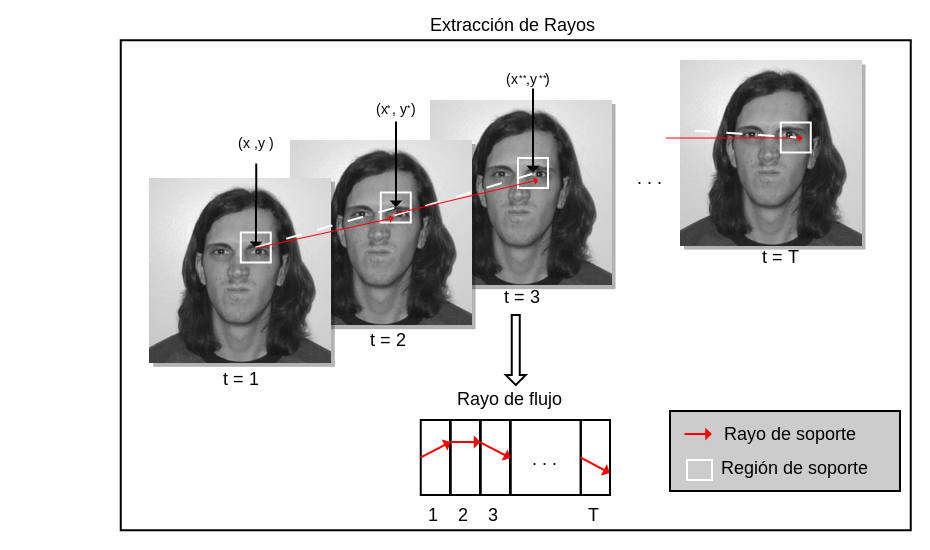
\includegraphics[width=9cm]{imagenes/Extraccion_de_rayos.png}
            \end{figure}             
            
            
        \end{frame}
       

        \begin{frame}{Extracción de micro-descriptores}{Normalización de rayos}
            \begin{figure}[bt]
        		\centering
                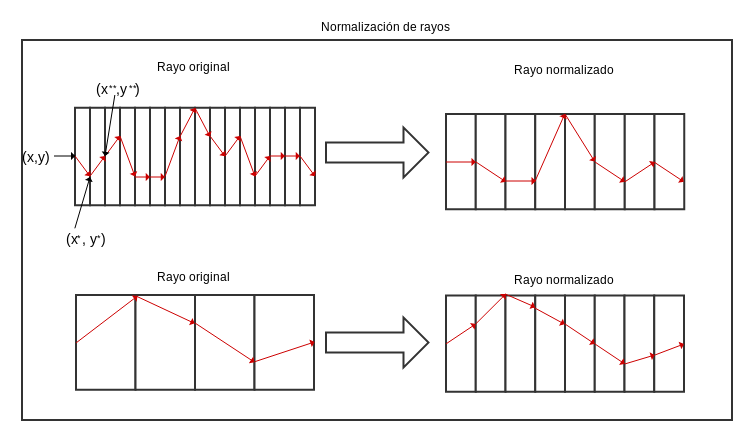
\includegraphics[width=10cm]{imagenes/normalizacion_de_rayos.png}
            \end{figure}
        \end{frame}
    
    \subsection{Creación de macro-descriptores}
		\begin{frame}{Creación de macro-descriptores}{Vista general}
            \begin{figure}[bt]
        		\centering
                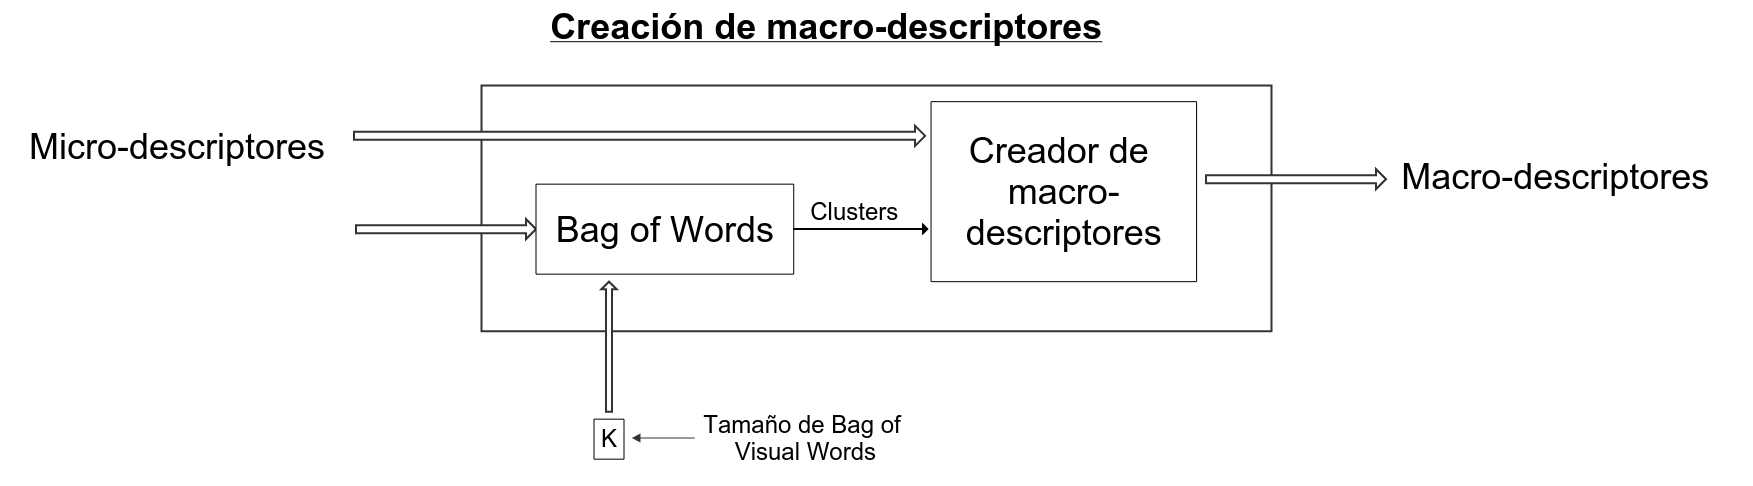
\includegraphics[width=8cm]{imagenes/Extractor_macrodescriptores_entrenamiento.png}
          		\caption{Creación de macro-descriptores entrenamiento.}
            \end{figure}
            
            \begin{figure}[bt]
        		\centering
                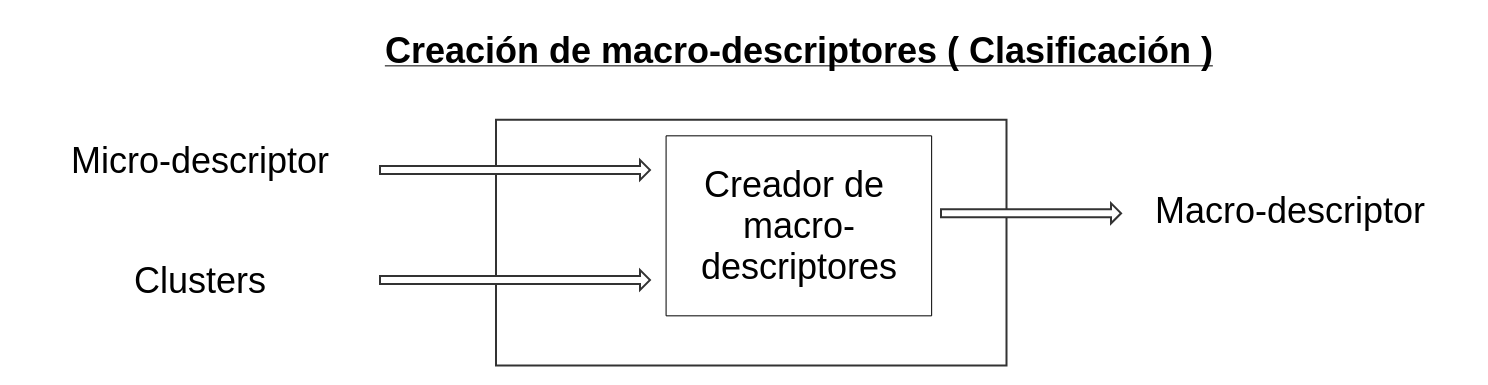
\includegraphics[width=8cm]{imagenes/Extractor_macrodescriptores_clasificacion.png}
          		\caption{Creación de macro-descriptores clasificador.}
            \end{figure}
        \end{frame}
        
        
        \begin{frame}{Creación de macro-descriptores}{Bag of Visual Words}
            \begin{equation}
  				\label{algoritmo:eq:dist}
				k^* = \arg \min_k \{\mathit{dist}(R(x,y),C_k)\},
			\end{equation}
            \begin{figure}[bt]
        		\centering
                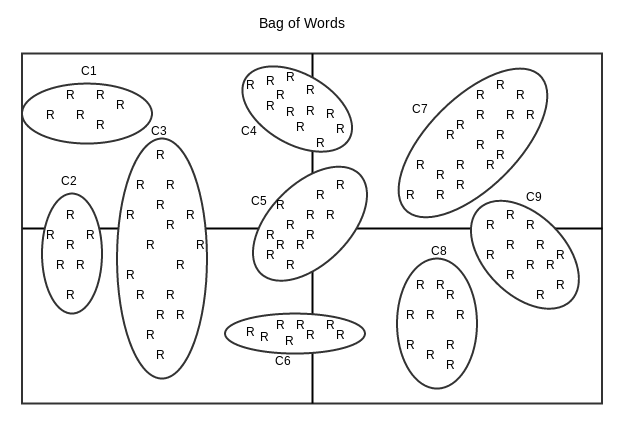
\includegraphics[width=7cm]{imagenes/bow_solo.png}
            \end{figure}
        \end{frame}
        
        \begin{frame}{Creación de macro-descriptores}{Creación del descriptor}
			\begin{equation}
				D_i(k) = \sum_{(x,y)\in\text{ROI}_i} \delta (R(x,y),k) \quad \forall k
			\end{equation}
			\begin{equation}
				 \delta (R(x,y),k) =  \begin{cases}
				 1 & \mbox{si }R(x,y)~\in~C_k\\
     			0 & \text{otro caso}
     			\end{cases}
			\end{equation}
		
			\begin{equation}
				\mathbb{D} = \cat_{i = 1}^{I} D_i, \quad \forall i
			\end{equation}				
			
			\begin{columns}[onlytextwidth]
                \begin{column}{0.3\textwidth}
				    \begin{figure}[tb]
        					\centering
                			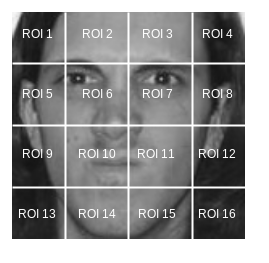
\includegraphics[width=3cm]{imagenes/rois.png}
            			\end{figure}
	        		\end{column}
            		\begin{column}{0.7\textwidth}
				    \begin{figure}[tb]
        					\centering
                			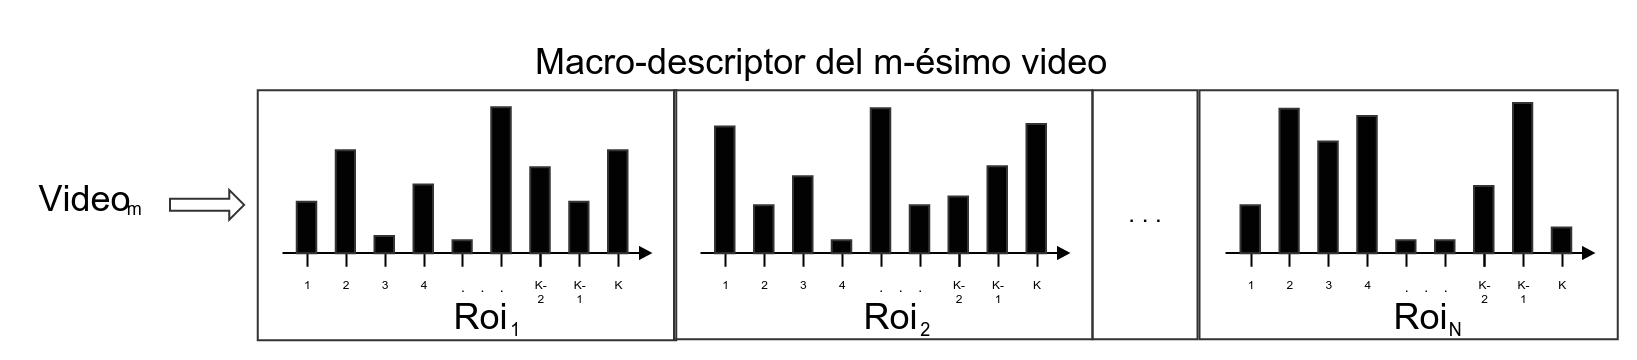
\includegraphics[width=7cm]{imagenes/macro-descriptor.png}
            			\end{figure}
            		\end{column}
            	\end{columns}
        \end{frame}
    \subsection{Entrenamiento y clasificación}
    


		%\begin{frame}{Entrenamiento y clasificación}{Support Vector Machines}
        %   \begin{figure}[bt]
        %	\centering
        %       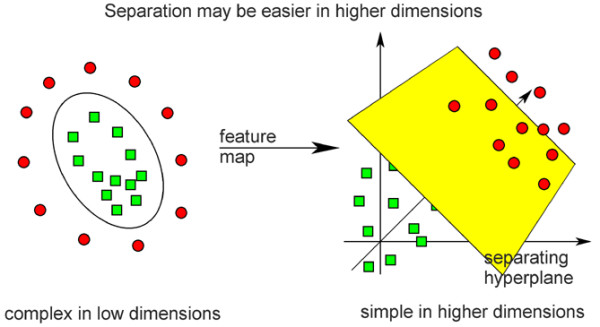
\includegraphics[width=8cm]{imagenes/svm.jpg}
        % 		\caption{Utilización de Kernel para el cambio de espacio.}
        %   \end{figure}
        %\end{frame}
        
        \begin{frame}{Entrenamiento y clasificación}{Support Vector Machines}
            \begin{figure}[bt]
        		\centering
                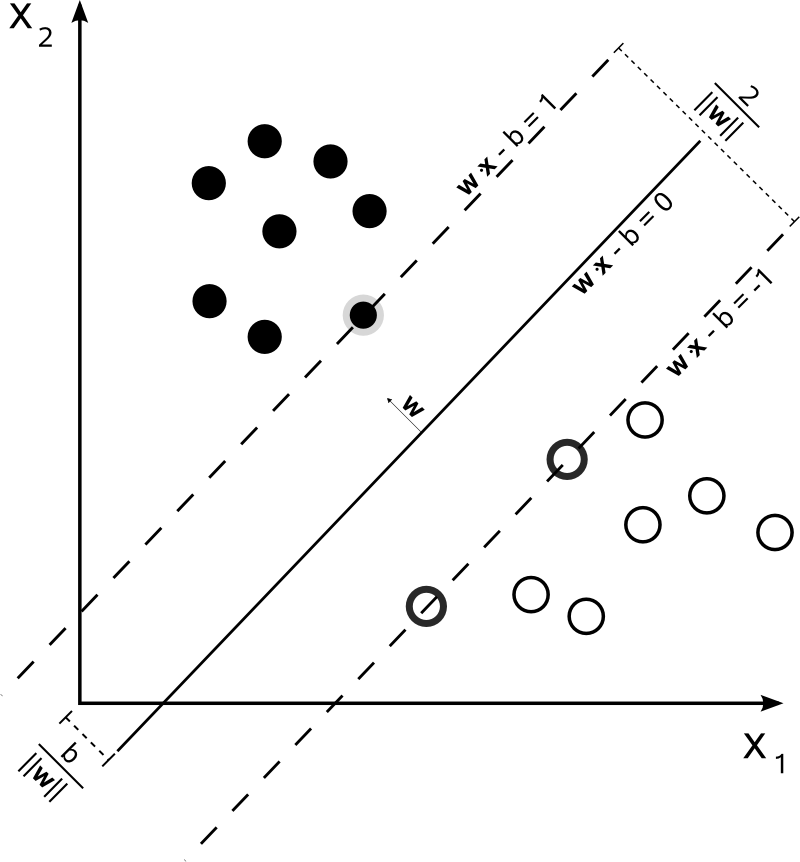
\includegraphics[width=5cm]{imagenes/support_vector_machines.png}
            \end{figure}
        \end{frame}
        
        \begin{frame}{Entrenamiento y clasificación}{k-fold cross validation}
            \begin{figure}[bt]
        		\centering
                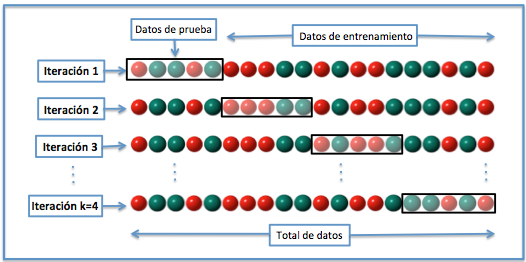
\includegraphics[width=7cm]{imagenes/K-fold.jpg}
            \end{figure}
            \begin{equation}
            		Accuracy = \frac{|Videos~bien~clasificados|}{|Total~de~videos|} 
            \end{equation}
   
        \end{frame}
        
        
	\subsection{Ventajas potenciales del método}
		\begin{frame}{Solución propuesta}{Preguntas a responder}
					
					\begin{itemize}
						\item ¿Permitirán los \textit{rayos} realizar un modelado espacio-temporal?
						\item ¿Los \textit{rayos de flujo} permitirán ver cual es el comportamiento de los pixeles a través del tiempo?
						\item ¿Permitirán los \textit{rayos} modelar micro-patrones en los movimientos del rostro que no pueden ser vistos a simple vista por los humanos?, de ser cierto, ¿estos micro-patrones aportarán mayor información al modelo de clasificación?.
						\item ¿Existe la posibilidad de que cada una de las expresiones faciales universales pueda tener asociado un conjunto de \textit{rayos} que la definan?. 
					\end{itemize}
		\end{frame}	

  \section{Experimentos}
  	\subsection{Base de datos}
  	\begin{frame}{Base de datos utilizada para los experimentos}{Base de datos MMI}
  		%\movie[[width=3cm,height=2cm]{}{videos/v1.avi}
  		\begin{center}
  			\includemedia[
  			width=0.7\linewidth,
  			height=0.6\linewidth,
  			activate=pageopen,
  			addresource=./videos/MMI.mp4,
  			flashvars={
  				source=./videos/MMI.mp4
  				& loop=true
  				& autoPlay=true
  				& autoRewind=true
  			}
  			]{}{VPlayer.swf}
  		\end{center}		
  	\end{frame}	
  
  
  	\subsection{Experimentos en la extracción de micro-descriptores}
  	\begin{frame}{Experimentos en la extracción de micro-descriptores}{Representación de los \textit{rayos de flujo} en el plano horizontal y vertical}
  		\definecolor{lightgray}{gray}{0.9}
  		\newlength{\sz}
  		\setlength{\sz}{1.7cm}
  		\begin{table}[t]
  			\centering
  			\begin{tabular}{ >{\centering\arraybackslash}m{.2cm}  >{\centering\arraybackslash}m{1.5cm}  >{\centering\arraybackslash}m{1.3cm}  >{\centering\arraybackslash}m{1.1cm}  >{\centering\arraybackslash}m{1.5cm}  >{\centering\arraybackslash}m{1.3cm}  >{\centering\arraybackslash}m{1.1cm}  }
  				\hline\noalign{\smallskip}
  				& \multicolumn{3}{ c }{Imágenes sin codificación} & \multicolumn{3}{ c }{Imágenes con LBP}\\
  				\hline\noalign{\smallskip}
  				\raisebox{.2cm}{\rotatebox{90}{\centering\parbox{1.7cm}{E1--Ira}}} & 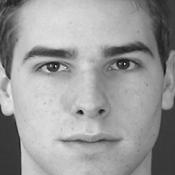
\includegraphics[height=\sz]{../Tesis/Figuras/resultados/E1/E1.png} & 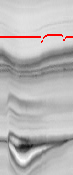
\includegraphics[height=\sz, angle=90]{../Tesis/Figuras/resultados/E1/E1_YT.png} & 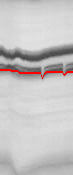
\includegraphics[height=\sz]{../Tesis/Figuras/resultados/E1/E1_XT.png} & 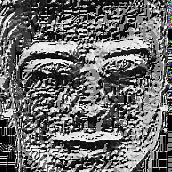
\includegraphics[height=\sz]{../Tesis/Figuras/resultados/E1/E1_LBP.png} & 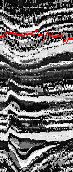
\includegraphics[height=\sz, angle=90]{../Tesis/Figuras/resultados/E1/E1_LBP_YT.png} & 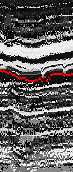
\includegraphics[height=\sz]{../Tesis/Figuras/resultados/E1/E1_LBP_XT.png} \\
  				
  				\raisebox{.2cm}{\rotatebox{90}{\centering\parbox{1.7cm}{E2--Asco}}}& 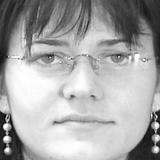
\includegraphics[height=\sz]{../Tesis/Figuras/resultados/E2/E2.png} & 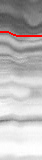
\includegraphics[height=\sz, angle=90]{../Tesis/Figuras/resultados/E2/E2_YT.png} & 
\includegraphics[height=\sz]{../Tesis/Figuras/resultados/E2/E2_XT.png} & 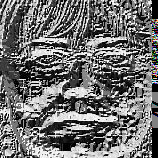
\includegraphics[height=\sz]{../Tesis/Figuras/resultados/E2/E2_LBP.png} & 
\includegraphics[height=\sz, angle=90]{../Tesis/Figuras/resultados/E2/E2_LBP_YT.png} & 
\includegraphics[height=\sz]{../Tesis/Figuras/resultados/E2/E2_LBP_XT.png} \\
  				
  				\raisebox{.3cm}{\rotatebox{90}{\centering\parbox{1.7cm}{E3--Miedo}}}& 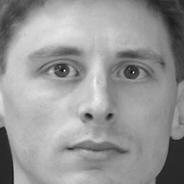
\includegraphics[height=\sz]{../Tesis/Figuras/resultados/E3/E3.png} & 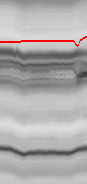
\includegraphics[height=\sz, angle=90]{../Tesis/Figuras/resultados/E3/E3_YT.png} & 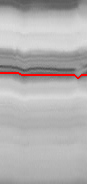
\includegraphics[height=\sz]{../Tesis/Figuras/resultados/E3/E3_XT.png} & 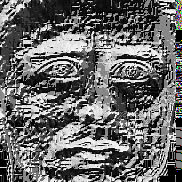
\includegraphics[height=\sz]{../Tesis/Figuras/resultados/E3/E3_LBP.png} & 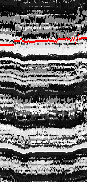
\includegraphics[height=\sz, angle=90]{../Tesis/Figuras/resultados/E3/E3_LBP_YT.png} & 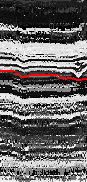
\includegraphics[height=\sz]{../Tesis/Figuras/resultados/E3/E3_LBP_XT.png} \\
  				&  & (XT) & (YT) &  & (XT) & (YT) \\
  				
  				
  			\end{tabular}
  			\label{tabla:comparacion_rayos1}
  		\end{table}
  		
  	\end{frame}	
  	\begin{frame}{Experimentos en la extracción de micro-descriptores}{Representación de los \textit{rayos de flujo} en el plano horizontal y vertical}
  		\setlength{\sz}{1.6cm}
  		\begin{table}[t]
  			\centering
  			\begin{tabular}{ >{\centering\arraybackslash}m{.2cm}  >{\centering\arraybackslash}m{1.4cm}  >{\centering\arraybackslash}m{1.4cm}  >{\centering\arraybackslash}m{1.1cm}  >{\centering\arraybackslash}m{1.4cm}  >{\centering\arraybackslash}m{1.4cm}  >{\centering\arraybackslash}m{1.1cm}  }
  				\hline\noalign{\smallskip}
  				& \multicolumn{3}{ c }{Imágenes sin codificación} & \multicolumn{3}{ c }{Imágenes con LBP}\\
  				\hline\noalign{\smallskip}	
  			
  				\raisebox{.2cm}{\rotatebox{90}{\centering\parbox{1.9cm}{E4--Alegría}}}& 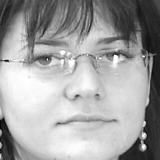
\includegraphics[height=\sz]{../Tesis/Figuras/resultados/E4/E4.png} & 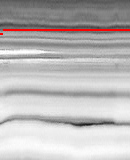
\includegraphics[height=\sz, angle=90]{../Tesis/Figuras/resultados/E4/E4_YT.png} & 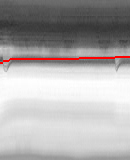
\includegraphics[height=\sz]{../Tesis/Figuras/resultados/E4/E4_XT.png} & 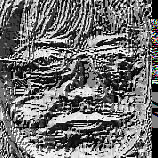
\includegraphics[height=\sz]{../Tesis/Figuras/resultados/E4/E4_LBP.png} & 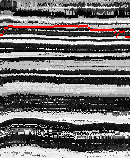
\includegraphics[height=\sz, angle=90]{../Tesis/Figuras/resultados/E4/E4_LBP_YT.png} & 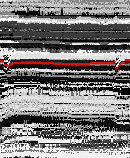
\includegraphics[height=\sz]{../Tesis/Figuras/resultados/E4/E4_LBP_XT.png} \\
  				
  				\raisebox{0cm}{\rotatebox{90}{\centering\parbox{1.9cm}{E5--Tristeza}}}& 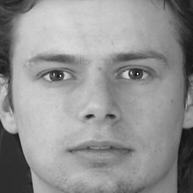
\includegraphics[height=\sz]{../Tesis/Figuras/resultados/E5/E5.png} & 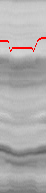
\includegraphics[height=\sz, angle=90]{../Tesis/Figuras/resultados/E5/E5_YT.png} & 
\includegraphics[height=\sz]{../Tesis/Figuras/resultados/E5/E5_XT.png} & 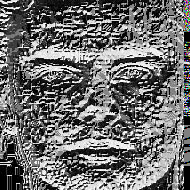
\includegraphics[height=\sz]{../Tesis/Figuras/resultados/E5/E5_LBP.png} & 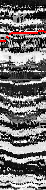
\includegraphics[height=\sz, angle=90]{../Tesis/Figuras/resultados/E5/E5_LBP_YT.png} & \includegraphics[height=\sz]{../Tesis/Figuras/resultados/E5/E5_LBP_XT.png} \\
  				
  				\raisebox{0cm}{\rotatebox{90}{\centering\parbox{2.1cm}{E6--Sorpresa}}}& \includegraphics[height=\sz]{../Tesis/Figuras/resultados/E6/E6.png} & \includegraphics[height=\sz, angle=90]{../Tesis/Figuras/resultados/E6/E6_YT.png} & \includegraphics[height=\sz]{../Tesis/Figuras/resultados/E6/E6_XT.png} & \includegraphics[height=\sz]{../Tesis/Figuras/resultados/E6/E6_LBP.png} & \includegraphics[height=\sz, angle=90]{../Tesis/Figuras/resultados/E6/E6_LBP_YT.png} & \includegraphics[height=\sz]{../Tesis/Figuras/resultados/E6/E6_LBP_XT.png} \\
  				&  & (XT) & (YT) &  & (XT) & (YT) \\
  				
  				
  			\end{tabular}
  			\label{tabla:comparacion_rayos2}
  		\end{table}
  		
  	\end{frame}
	
	\begin{frame}{Experimentos en la extracción de micro-descriptores}{Cálculo de error del modelado de los \textit{rayos de flujo} en el plano horizontal y vertical}
		\begin{table}[t]
			\centering
			\begin{tabular}{ >{\centering\arraybackslash}m{2.0cm}  >{\centering\arraybackslash}m{1.2cm}  >{\centering\arraybackslash}m{1.2cm}  >{\centering\arraybackslash}m{1.2cm}  >{\centering\arraybackslash}m{1.2cm}  >{\centering\arraybackslash}m{1.2cm}  >{\centering\arraybackslash}m{1.2cm} }
				\hline
				Codificación & \multicolumn{3}{ c }{XT} & \multicolumn{3}{ c }{YT}\\
				\hline
				& & & & & &\\
				Sin codificación & \includegraphics[width=1.2cm]{../Tesis/Figuras/resultados/comparacion_real/no_lbp/YT/extraido.png} & \includegraphics[width=1.2cm]{../Tesis/Figuras/resultados/comparacion_real/no_lbp/YT/pintado.png} & \includegraphics[width=1.2cm]{../Tesis/Figuras/resultados/comparacion_real/no_lbp/YT/superposicion.png} & \includegraphics[width=1.2cm]{../Tesis/Figuras/resultados/comparacion_real/no_lbp/XT/extraido.png} & \includegraphics[width=1.2cm]{../Tesis/Figuras/resultados/comparacion_real/no_lbp/XT/pintado.png} & \includegraphics[width=1.2cm]{../Tesis/Figuras/resultados/comparacion_real/no_lbp/XT/superposicion.png} \\
				
				Codificación LBP & \includegraphics[width=1.2cm]{../Tesis/Figuras/resultados/comparacion_real/lbp/YT/extraido.png} & \includegraphics[width=1.2cm]{../Tesis/Figuras/resultados/comparacion_real/lbp/YT/pintado.png} & \includegraphics[width=1.2cm]{../Tesis/Figuras/resultados/comparacion_real/lbp/YT/superposicion.png} & \includegraphics[width=1.2cm]{../Tesis/Figuras/resultados/comparacion_real/lbp/XT/extraido.png} & \includegraphics[width=1.2cm]{../Tesis/Figuras/resultados/comparacion_real/lbp/XT/pintado.png} & \includegraphics[width=1.2cm]{../Tesis/Figuras/resultados/comparacion_real/lbp/XT/superposicion.png} \\
				
				& (i) & (ii) & (iii) & (iv) & (v) & (vi)\\
				
			\end{tabular}
			\label{tabla:comparacion_errores}
		\end{table}
	\end{frame}
	\pgfplotstableset{
		franjas/.style={
			columns/errorG/.style={
				column name=Error,
				precision=1
			},
			every even row/.style={
				before row={\rowcolor{#1}}
			},
			every head row/.style={
				before row=\hline\noalign{\smallskip},after row=\hline
			},
			every last row/.style={
				after row=\hline
			},
			set decimal separator={,},
		},
		franjas/.default={gray!50},
		tablita/.style={
			columns={rs, ws, errorYT, errorXT, errorG},
			columns/rs/.style={
				column name=$RS$,
			},
			columns/ws/.style={
				column name=$WS$,
			},
			columns/errorXT/.style={
				column name=Error vertical,
				precision=1
			},
			columns/errorYT/.style={
				column name=Error horizontal,
				precision=1
			},
			franjas,
		},
		tablaK/.style={
			columns={N, K, Accuracy},
			columns/N/.style={
				column name=$N$,
			},
			columns/K/.style={
				column name=$K$,
			},
			columns/Accuracy/.style={
				column name=Accuracy,
				precision=1,
				postproc cell content/.append style={
					/pgfplots/table/@cell content/.add={}{\,\%}
				}
			},
			franjas,
		},
		tablaN/.style={
			columns={RS, WS, N, Accuracy},
			columns/RS/.style={
				column name=$RS$,
			},
			columns/WS/.style={
				column name=$WS$,
			},
			columns/N/.style={
				column name=$N$,
			},
			columns/Accuracy/.style={
				column name=Accuracy,
				precision=1,
				postproc cell content/.append style={
					/pgfplots/table/@cell content/.add={}{\,\%}
				}
			},
			franjas,
		},
		tablaSVMresultsRBF/.style={
			columns={Gamma,C-value,Accuracy},
			columns/Gamma/.style={
				column name=$Gamma$,
				precision=3
			},
			columns/C-value/.style={
				column name=$C-value$,
				precision=3
			},
			columns/Accuracy/.style={
				column name=$Accuracy$,
				precision=1,
				postproc cell content/.append style={
					/pgfplots/table/@cell content/.add={}{\,\%}
				}
			},
			franjas,
		},
		tablaSVMresultsLineal/.style={
			columns={C-value,Accuracy},
			columns/C-value/.style={
				column name=$C-value$,
				precision=3
			},
			columns/Accuracy/.style={
				column name=$Accuracy$,
				precision=1,
				postproc cell content/.append style={
					/pgfplots/table/@cell content/.add={}{\,\%}
				}
			},
			franjas,
		},
		tablaSVMresultsPoly/.style={
			columns={Degree,Gamma,C-value,Accuracy},
			columns/Degree/.style={
				column name=$Degree$,
			},
			columns/Gamma/.style={
				column name=$Gamma$,
				precision=3
			},
			columns/C-value/.style={
				column name=$C-value$,
				precision=3
			},
			columns/Accuracy/.style={
				column name=$Accuracy$,
				precision=1,
				postproc cell content/.append style={
					/pgfplots/table/@cell content/.add={}{\,\%}
				}
			},
			franjas,
		},
		tablaSVMresults/.style={
			columns={RS,WS,N,K,Accuracy},
			columns/RS/.style={
				column name=$RS$,
			},
			columns/WS/.style={
				column name=$WS$,
			},
			columns/N/.style={
				column name=$N$,
			},
			columns/K/.style={
				column name=$K$,
			},
			columns/Accuracy/.style={
				column name=$Accuracy$,
				precision=1,
				postproc cell content/.append style={
					/pgfplots/table/@cell content/.add={}{\,\%}
				}
			},
			franjas,
		},
		tablaSVMresultscmp/.style={
			columns={Autor,K-fold,Accuracy},
			columns/Accuracy/.style={
				column name=$Accuracy$,
				precision=1,
				postproc cell content/.append style={
					/pgfplots/table/@cell content/.add={}{\,\%}
				}
			},
			franjas,
		},
	}
	
	\begin{frame}{Experimentos en la extracción de micro-descriptoress}{Cálculo de error del modelado de los \textit{rayos de flujo} en el plano horizontal y vertical}
		\begin{table}[tb]
			\centering
			\pgfplotstabletypeset[tablita]{../Tesis/Datos/comparacion_NO_LBP.dat}
			\caption{Error calculado sin codificación LBP.}
			\label{tabla:error_no_lbp}
		\end{table}
	\end{frame}
	
	\begin{frame}{Experimentos en la extracción de micro-descriptores}{Cálculo de error del modelado de los \textit{rayos de flujo} en el plano horizontal y vertical}
		\begin{table}[tb]
			\centering
			\pgfplotstabletypeset[tablita]{../Tesis/Datos/comparacion_LBP.dat}
			\caption{Error calculado con codificación LBP.}
			\label{tabla:error_lbp}
		\end{table}
	\end{frame}


	\begin{frame}{Experimentos en la extracción de micro-descriptores}{Modelado de \textit{rayos de flujo} en videos sintéticos sin textura}
		%\movie[[width=3cm,height=2cm]{}{videos/v1.avi}
		\begin{center}
			\includemedia[
			width=0.7\linewidth,
			height=0.6\linewidth,
			activate=pageopen,
			addresource=./videos/v1.mp4,
			flashvars={
				source=./videos/v1.mp4
				& loop=true
				& autoPlay=true
				& autoRewind=true
				}
				]{}{VPlayer.swf}
		\end{center}		
	\end{frame}	
	
	\begin{frame}{Experimentos en la extracción de micro-descriptores}{Modelado de \textit{rayos de flujo} en videos sintéticos con textura}
		%\movie[[width=3cm,height=2cm]{}{videos/v1.avi}
		\begin{center}
			\includemedia[
			width=0.7\linewidth,
			height=0.6\linewidth,
			activate=pageopen,
			addresource=./videos/v2.mp4,
			flashvars={
				source=./videos/v2.mp4
				& loop=true
				& autoPlay=true
			}
			]{}{VPlayer.swf}
		\end{center}		
	\end{frame}	
	
	\begin{frame}{Experimentos en la extracción de micro-descriptores}{Modelado de \textit{rayos de flujo} en videos sintéticos con textura y distintos movimientos}
		%\movie[[width=3cm,height=2cm]{}{videos/v1.avi}
		\begin{center}
			\includemedia[
			width=0.7\linewidth,
			height=0.6\linewidth,
			activate=pageopen,
			addresource=./videos/v3.mp4,
			flashvars={
				source=./videos/v3.mp4
				& loop=true
			}
			]{}{VPlayer.swf}
		\end{center}		
	\end{frame}	
	
	\subsection{Experimentos en la creación de macro-descriptores}
	\begin{frame}{Experimentos en la creación de macro-descriptores}{Representación visual de distribución de \textit{clusters} en el rostro}
		\newlength{\st}
		\setlength{\st}{1.4cm}
		\setlength{\sz}{1.5cm}
		\begin{table}[tb]
			\centering
			\begin{tabular}{ >{\centering\arraybackslash}m{.5cm}  >{\centering\arraybackslash}m{\st}  >{\centering\arraybackslash}m{\st}  >{\centering\arraybackslash}m{\st}  >{\centering\arraybackslash}m{\st}  >{\centering\arraybackslash}m{\st}  >{\centering\arraybackslash}m{\st}  }
				\hline\noalign{\smallskip}
				$K$ & Ira & Asco & Miedo & Alegría & Tristeza & Sorpresa\\
				\hline\noalign{\smallskip}
				10 & \includegraphics[height=\sz]{../Tesis/Figuras/resultados/clustering/k=10/E1_ec.png} & \includegraphics[height=\sz]{../Tesis/Figuras/resultados/clustering/k=10/E2_ec.png} & \includegraphics[height=\sz]{../Tesis/Figuras/resultados/clustering/k=10/E3_ec.png} & \includegraphics[height=\sz]{../Tesis/Figuras/resultados/clustering/k=10/E4_ec.png} & \includegraphics[height=\sz]{../Tesis/Figuras/resultados/clustering/k=10/E5_ec.png} & \includegraphics[height=\sz]{../Tesis/Figuras/resultados/clustering/k=10/E6_ec.png} \\
				
				50 & \includegraphics[height=\sz]{../Tesis/Figuras/resultados/clustering/k=50/E1_ec.png} & \includegraphics[height=\sz]{../Tesis/Figuras/resultados/clustering/k=50/E2_ec.png} & \includegraphics[height=\sz]{../Tesis/Figuras/resultados/clustering/k=50/E3_ec.png} & \includegraphics[height=\sz]{../Tesis/Figuras/resultados/clustering/k=50/E4_ec.png} & \includegraphics[height=\sz]{../Tesis/Figuras/resultados/clustering/k=50/E5_ec.png} & \includegraphics[height=\sz]{../Tesis/Figuras/resultados/clustering/k=50/E6_ec.png} \\
				
				100 & \includegraphics[height=\sz]{../Tesis/Figuras/resultados/clustering/k=100/E1_ec.png} & \includegraphics[height=\sz]{../Tesis/Figuras/resultados/clustering/k=100/E2_ec.png} & \includegraphics[height=\sz]{../Tesis/Figuras/resultados/clustering/k=100/E3_ec.png} & \includegraphics[height=\sz]{../Tesis/Figuras/resultados/clustering/k=100/E4_ec.png} & \includegraphics[height=\sz]{../Tesis/Figuras/resultados/clustering/k=100/E5_ec.png} & \includegraphics[height=\sz]{../Tesis/Figuras/resultados/clustering/k=100/E6_ec.png} \\
				
				& (E1) & (E2) & (E3) & (E4) & (E5) & (E6) \\
			\end{tabular}
			%\caption{Tabla comparativa de la cantidad de \textit{cluster} utilizados y su representación en las distintas expresiones faciales. Las imágenes fueron construidas en escala de grises, los colores mas cercanos al blanco representan mayor cantidad de \textit{rayos} agrupados en ese conjunto. }
			\label{tabla:comparacion_clusters1} 
		\end{table}
	\end{frame}
	
	\begin{frame}{Experimentos en la creación de macro-descriptores}{Representación visual de distribución de \textit{clusters} en el rostro}
		\setlength{\st}{1.4cm}
		\setlength{\sz}{1.5cm}
		\begin{table}[tb]
			\centering
			\begin{tabular}{ >{\centering\arraybackslash}m{.5cm}  >{\centering\arraybackslash}m{\st}  >{\centering\arraybackslash}m{\st}  >{\centering\arraybackslash}m{\st}  >{\centering\arraybackslash}m{\st}  >{\centering\arraybackslash}m{\st}  >{\centering\arraybackslash}m{\st}  }
				\hline\noalign{\smallskip}
				$K$ & Ira & Asco & Miedo & Alegría & Tristeza & Sorpresa\\
				\hline\noalign{\smallskip}

				500 & \includegraphics[height=\sz]{../Tesis/Figuras/resultados/clustering/k=500/E1_ec.png} & \includegraphics[height=\sz]{../Tesis/Figuras/resultados/clustering/k=500/E2_ec.png} & \includegraphics[height=\sz]{../Tesis/Figuras/resultados/clustering/k=500/E3_ec.png} & \includegraphics[height=\sz]{../Tesis/Figuras/resultados/clustering/k=500/E4_ec.png} & \includegraphics[height=\sz]{../Tesis/Figuras/resultados/clustering/k=500/E5_ec.png} & \includegraphics[height=\sz]{../Tesis/Figuras/resultados/clustering/k=500/E6_ec.png} \\
				
				1000 & \includegraphics[height=\sz]{../Tesis/Figuras/resultados/clustering/k=1000/E1_ec.png} & \includegraphics[height=\sz]{../Tesis/Figuras/resultados/clustering/k=1000/E2_ec.png} & \includegraphics[height=\sz]{../Tesis/Figuras/resultados/clustering/k=1000/E3_ec.png} & \includegraphics[height=\sz]{../Tesis/Figuras/resultados/clustering/k=1000/E4_ec.png} & \includegraphics[height=\sz]{../Tesis/Figuras/resultados/clustering/k=1000/E5_ec.png} & \includegraphics[height=\sz]{../Tesis/Figuras/resultados/clustering/k=1000/E6_ec.png} \\

				& (E1) & (E2) & (E3) & (E4) & (E5) & (E6) \\
			\end{tabular}
			%\caption{Tabla comparativa de la cantidad de \textit{cluster} utilizados y su representación en las distintas expresiones faciales. Las imágenes fueron construidas en escala de grises, los colores mas cercanos al blanco representan mayor cantidad de \textit{rayos} agrupados en ese conjunto. }
			\label{tabla:comparacion_clusters2} 
		\end{table}
	\end{frame}
				
	\subsection{Experimentos generales del algoritmo}
	
	\begin{frame}{Experimentos generales del algoritmo}{Comparativa con otros métodos del estado del arte}
		\begin{table}[tb]
			\centering
			\begin{tabular}{l c}
				\hline
				Autor & \textit{Accuracy}\\
				\hline
				
				\rowcolor{gray!50} 
				\/[Yeasin \emph{et al}., 2004\/] & 90,0 \% \\
				
				\/[Xiang \emph{et al}., 2008\/] & 88,8 \%\\
				
				\rowcolor{gray!50} 
				\/[Buenaposada \emph{et al}., 2008\/] & 89,1 \%\\
				
				\/[Zhao y Pietikäinen, 2007\/]~a & 95,1 \%\\
				
				\rowcolor{gray!50} 
				\/[Zhao y Pietikäinen, 2007\/]~b & 93,8 \%\\
				
				\/[Ji y Idrissi, 2012\/] LBP & 91,6 \%\\
				
				\rowcolor{gray!50} 
				\/[Ji y Idrissi, 2012\/] LBP + VTB & 93,6 \%\\
				
				\/[Ji y Idrissi, 2012\/] Moments & 98,5 \%\\
				
				\rowcolor{gray!50} 
				\textit{Rayos de flujo} & 48,6 \%\\
				\hline
			\end{tabular}
			\caption{Tabla comparativa de resultados obtenidos con distintos métodos en el estado del arte.}
			\label{tabla:exp:accuracy_cmp}
		\end{table}
	\end{frame}
			     
  \section{Conclusiones}
  	\begin{frame}{Conclusiones}{Preguntas planteadas}
  		\begin{itemize}
  			\item ¿Permitirán los \textit{rayos} realizar un modelado espacio-temporal?
  			\item ¿Los \textit{rayos de flujo} permitirán ver cual es el comportamiento de los pixeles a través del tiempo?
  			\item ¿Permitirán los \textit{rayos} modelar micro-patrones en los movimientos del rostro que no pueden ser vistos a simple vista por los humanos?, de ser cierto, ¿estos micro-patrones aportarán mayor información al modelo de clasificación?
  			\item ¿Existe la posibilidad de que cada una de las expresiones faciales universales pueda tener asociado un conjunto de \textit{rayos} que la definan?
  		\end{itemize}
  	\end{frame}
  
	\begin{frame}{Conclusiones}{Conclusiones generales}
		\begin{itemize}
			\item Aproximación al movimiento de los pixeles.
			\item Tamaño de la RS y WS.
			\item Texturas de la imagen del rostro son de vital importancia.
			\item Ruido por extracción en regiones que no aportan información.
			\item \textit{Clustering} localizado en regiones importantes del rostro.
			\item Utilizar solo regiones del rostro: nariz, boca, ceja, etc
			
		\end{itemize}
	\end{frame}      

\section{Trabajos futuros}
        \begin{frame}{Trabajos futuros}{Experimentos}
			\begin{enumerate}
				\item Utilizar solo la variable vertical
				\item Utilizar el angulo de movimiento
				\item Utilizar solo regiones importantes del rostro (Nariz, boca, ojos y cejas)
				\item Mezclar con FACS de Ekman
			\end{enumerate}					        
        \end{frame}
    

% All of the following is optional and typically not needed. 

\begin{frame}
	\frametitle{Referencias}
	\footnotesize{
		\begin{thebibliography}{99} % Beamer does not support BibTeX so references must be inserted manually as below
			
			\bibitem[Yeasin et al., 2004]{Yeasin2004} Yeasin~\emph{et al} (2004).
			\newblock From facial expression to level of interest: a spatio-temporal approach
			\newblock Proceedings of the 2004 IEEE Computer Society Conference on Computer Vision and Pattern Recognition, 2004.
			
			\bibitem[Zhao y Pietikäinen, 2007]{Zhao2007} Zhao y Pietikäinen (2007).
			\newblock Dynamic Texture Recognition Using Local Binary Patterns with an Application to Facial Expressions
			\newblock \emph{IEEE Transactions on Pattern Analysis and Machine Intelligence} 29(6), 915 -- 928.
			
			
			\bibitem[Xiang et al., 2008]{Xiang2008} Xiang~\emph{et al} (2008).
			\newblock Expression recognition using fuzzy spatio-temporal modeling
			\newblock \emph{Pattern Recognition} 41(1), 204 -- 216.
			
			\bibitem[Buenaposada et al., 2008]{Buenaposada2008} Buenaposada~\emph{et al} (2008).
			\newblock Recognising facial expressions in video sequences
			\newblock \emph{Pattern Analysis and Applications} 11(1), 101 -- 116.
			
			\bibitem[Ji y Idrissi, 2012]{Ji2012} Ji y Idrissi (2012)
			\newblock Automatic facial expression recognition based on spatiotemporal descriptors
			\newblock \emph{Pattern Recognition Letters} 33(10), 1373 -- 1380.
			
			
		\end{thebibliography}
	}
\end{frame}


\section*{Preguntas}
	\begin{frame}{Gracias por su atención}
		\begin{center}
			¿Preguntas?
		\end{center}
	\end{frame}

\section*{Anexo}
	\begin{frame}{Anexo I}{Definiciones}
		\begin{block}{Región de soporte}
                  Dado un píxel $(x,y)$ en un cuadro $t$, definimos una región de soporte RS, de tamaño $L \times L$ (donde $L$ es impar), como la subregión del cuadro $t$ que está centrada en el píxel $(x,y)$.
         \end{block}
         \begin{block}{Ventana de búsqueda}
                  Dado un píxel $(x,y)$ en un cuadro $t$, definimos la ventana de búsqueda WS, de  tamaño $(2L+1) \times (2L+1)$, como la subregión del cuadro $t+1$ que está centrada en el píxel $(x,y)$.
         \end{block}
    	\end{frame}
	\begin{frame}{Anexo I}{Definiciones}
		\begin{block}{Rayo de soporte}
                Dado un par ordenado $(x,y)$ en el tiempo $t$, el \textit{Rayo de soporte} para dicho píxel esta definido por el nuevo par ordenado $(\Delta x^{t}, \Delta y^{t})$, de tal forma que,
			\begin{equation}
				\rho_{(x,y)} = \{(\Delta x^{t}, \Delta y^{t})~| \forall t\}.
			\end{equation}		 
        \end{block}   
    \end{frame}
	\begin{frame}{Anexo I}{Definiciones}
	    \begin{block}{Rayo de flujo}
                Es el conjunto de \textit{Rayos de soporte} que representan el movimiento del píxel $(x,y)$ en cada uno de los cuadros $t$, este conjunto es definido como \textit{Rayo de flujo} o micro-descriptor, de tal forma que,
			\begin{equation}
				R(x,y)	 = \{\rho_{(x,y)}, \rho_{(x^*,y^*)}, \rho_{(x^{**},y^{**})}, ... \},
			\end{equation}
		donde ($x^{**}$,$y^{**}$) es el píxel al cual se desplazo ($x^{*}$,$y^{*}$) en el cuadro $t+2$.  
        \end{block}      
    \end{frame}	

	\begin{frame}{Anexo II}{Entrenamiento y clasificación}
  		\begin{columns}[onlytextwidth]
  	 			\begin{column}{0.5\textwidth}
          \begin{figure}[bt]
   			    			\centering
           		    		\includegraphics[width=6cm]{imagenes/Entrenamiento.png}
         				\caption{Diagrama de entrenamiento.}
           			\end{figure}
				\end{column}
   				\begin{column}{0.5\textwidth}
          \begin{figure}[bt]
       					\centering
       		        		\includegraphics[width=6cm]{imagenes/Clasificacion.png}
       	  				\caption{Diagrama de clasificación.}
          \end{figure}
       			\end{column}
	  \end{columns}
    \end{frame}

	\begin{frame}{Anexo III: Tipos de metodos}{Métodos Geométricos}
		\begin{columns}[onlytextwidth]
			\begin{column}{0.5\textwidth}
				\begin{figure}[bt]
					\centering
					\includegraphics[width=4cm]{imagenes/geo1.jpg}
				\end{figure}	
			\end{column}
			\begin{column}{0.5\textwidth}
				\begin{figure}[bt]
					\centering
					\includegraphics[width=4cm]{imagenes/geo2.jpg}
				\end{figure}	
			\end{column}
		\end{columns}      			
	\end{frame}
	
	\begin{frame}{Anexo III: Tipos de metodos}{Métodos de apariencia: Local Binary Patterns}
		\begin{figure}[bt]
			\centering
			\includegraphics[width=9cm]{imagenes/lbp.pdf}
		\end{figure}	
		
		\begin{figure}[bt]
			\centering
			\includegraphics[width=9cm]{imagenes/lbp_histogram.png}
		\end{figure}	  
	\end{frame}
	
	\begin{frame}{Anexo III: Tipos de metodos}{Métodos de apariencia: Local Direccional Number Patterns}
		\begin{figure}[bt]
			\centering
			\includegraphics[width=10cm]{imagenes/ldn.jpg}
		\end{figure}
	\end{frame}
	
	
	\begin{frame}{Anexo III: Tipos de metodos}{Métodos de apariencia: Volume Local Binary Patterns}
		\begin{figure}[bt]
			\centering
			\includegraphics[width=7cm]{imagenes/vlbp.pdf}
		\end{figure}
	\end{frame}
	
	
	\begin{frame}{Anexo III: Tipos de metodos}{Métodos de apariencia: Local Binary Patterns- Three Ortogonal Planes}
		\begin{figure}[bt]
			\centering
			\includegraphics[width=10cm]{imagenes/lbptop.pdf}
		\end{figure}
	\end{frame}
	
	\begin{frame}{Anexo IV: Resultados}{Resultados para elección del tamaño de la variable de normalización}
		\begin{table}[Bt]
			\centering
			\pgfplotstabletypeset[tablaN]{../Tesis/Figuras/resultados/Normalizacion/Accuracy_n.dat}
			\caption{Tabla comparativa del \textit{Accuracy} obtenido utilizando distintos valores de $N$ y distintos tamaños de las ventanas.}
			\label{tabla:accuracy_N}
		\end{table}
	\end{frame}
	
	\begin{frame}{Anexo IV: Resultados}{Resultados para la elección de la cantidad de \textit{clusters}}
		\begin{table}[tb]
			\centering
			\pgfplotstabletypeset[tablaK]{../Tesis/Figuras/resultados/clustering/Accuracy_k.dat}
			\caption{Tabla comparativa del \textit{Accuracy} obtenido utilizando distintos valores de $K$.}
			\label{tabla:accuracy_K}
		\end{table}
	\end{frame}
	
	
	\begin{frame}{Anexo IV: Resultados}{Eleccion de Kernel para SVM}
		\begin{table}[b]
			\centering
			\pgfplotstabletypeset[tablaSVMresultsRBF]{../Tesis/Datos/rbf_10.csv}
			\caption{Mejores resultados obtenidos por el Kernel RBF.}
			\label{tabla:svm_rbf}
		\end{table}
	\end{frame}
	
	
	\begin{frame}{Anexo IV: Resultados}{Elección de Kernel para SVM}
		\begin{table}[tb]
			\centering
			\pgfplotstabletypeset[tablaSVMresultsLineal]{../Tesis/Datos/lineal_10.csv}
			\caption{Mejores resultados obtenidos por el Kernel Lineal.}
			\label{tabla:svm_lineal}
		\end{table}
	\end{frame}
	
	\begin{frame}{Anexo IV: Resultados}{Elección de Kernel para SVM}
		\begin{table}[tb]
			\centering
			\pgfplotstabletypeset[tablaSVMresultsPoly]{../Tesis/Datos/poly_10.csv}
			\caption{Mejores resultados obtenidos por el Kernel Polinomial.}
			\label{tabla:svm_poly}
		\end{table}
	\end{frame}
	
	\begin{frame}{Anexo IV: Resultados}{Mejores resultados del algoritmo}
		\begin{table}[bt]
			\centering
			\pgfplotstabletypeset[tablaSVMresults]{../Tesis/Datos/resultados.dat}
			\caption{Resultados obtenidos utilizando las mejores variables obtenidas en el proceso de experimentos.}
			\label{tabla:exp:accuracy}
		\end{table}
	\end{frame}
	
\end{document}


